\section{Study 3: Design Interventions to Reduce Attrition}

Study 1 and Study 2 collectively demonstrated that rotation increases effectiveness but also increases attrition. Why does rotation increase attrition? To understand this, we needed to understand why users uninstalled in the first place.

We performed a qualitative content analysis on the uninstall feedback left to us by users. This feedback was collected in a tab that opened automatically when users uninstalled HabitLab. \rev{The page stated that feedback would be used for research purposes.} Users had the option to check boxes to agree with a set of predefined reasons they why they were uninstalling, and leave free-text feedback. We performed an inductive analysis of the free-text feedback, grouping responses by themes, reflecting on our themes, and refining our groupings until convergence.

% 43 of the users who submitted the form were exposed to one of the conditions of study 1
% 101 of the users who submitted the form were exposed to one of the conditions of study 2

% A total of 782 users have submitted the uninstall feedback form over the course of HabitLab's deployment. This includes 8 participants from Study 1, and 39 from Study 2.
% https://v2.overleaf.com/17562771pkwbxzxyvtvv
A total of 782 users submitted the uninstall feedback form. This data represents all past users of HabitLab, and includes users outside studies 1 and 2. We use this larger dataset because only 8 participants from Study 1, and 39 from Study 2, filled out the feedback form. 751 users who submitted the form checked at least one of our predefined reasons. 274 users (36\%) uninstalled because ``Interventions were annoying'', 248 users (33\%) uninstalled because HabitLab ``Did not feel effective'', 100 users (13\%) uninstalled because HabitLab ``Was causing lag'', 75 (10\%) uninstalled due to ``Privacy concerns'', and 202 (27\%) cited ``Other reasons''. The total sums to more than 100\% because users could check more than one reason.

A total 155 users submitted free-form textual feedback. Some users began with an incorrect mental model and uninstalled after they learned what it was doing:
\begin{itemize}
%\item \textit{does not f***ing work, hiding the newsfeed in particular} [The ``hide news feed'' intervention was advertised on the HabitLab Chrome store page, but HabitLab never hit that intervention in its rotation for this user before they uninstalled]
\item \textit{Didn't seem what I was expected. Installed two minutes ago and removed it}
\item \textit{I just didn't understand the concept before downloading} %and it's [sic] intentions aren't my demons as it happens}
\end{itemize}

Some users indicated they wanted more control over the intervention that was shown to them, or were simply looking for a time tracker and were not interested in interventions at all:
\begin{itemize}
\item \textit{I wanted a timer for every ``domain'', it can be good for statistics of time}
\item \textit{I was interested in tracking my usage to start, instead of setting interventions that I may not actually be concerned about}
% \item \textit{Would have preferred a gentle log - perhaps emailed - giving usage statistics. In present form this operates like pop-up ads. Still, it was reasonably insightful into understanding my usage for the time I used it}
\end{itemize}

Some users indicated dissatisfaction with particular interventions:
\begin{itemize}
\item \textit{Mostly it was the bar covering up facebook message indicators}
%\item \textit{You covered up useful buttons. Don't do that}
% \item \textit{Made Facebook unusable. Which might be the point?}
\item \textit{it was just annoying you out of not using sites, not convincing you to. It became like ads, they are always there. But you don't like them and turn them off with ad-block.}

\end{itemize}

Some users wished interventions would be more forceful, or less intrusive:
\begin{itemize}
\item \textit{Interventions are not forceful enough. They are too easy to click around or disable}
% \item \textit{Looked like some nice options for streamlining sites, but it's actually a nanny. I don't need a nanny whining at me.}
\item \textit{I liked the interventions but not on every page change or load, that was just a bit too much}
\end{itemize}

Finally, some users decided they simply did not want or need interventions:
\begin{itemize}
\item \textit{Made me realize I don't have Facebook addiction, spending less than 30 minutes [...] per day} %of my desktop time on it per day}
\item \textit{I'm weak...}
\end{itemize}


Other themes included localization issues, performance issues, privacy concerns, accidental installations, and misattribution of other issues to HabitLab.

\begin{comment}
Some feedback indicated that users had an incorrect mental model of the system: they were expecting to see a particular intervention consistently, instead of having them rotate:

\textit{does not fucking work, hiding the newsfeed in particular}

Other users began with an incorrect mental model and uninstalled after they learned what it was doing:

\textit{Didn't seem what I was expected. Installed two minutes ago and removed it}

\textit{I just didn't understand the concept before downloading and it's intentions aren't my demons as it happens}

Some users indicated they wanted more control over the intervention that was shown to them, or were simply looking for a time tracker and were not interested in interventions at all:

\textit{I wanted a timer for every "domain", it can be good for statistics of time}

\textit{I was interested in tracking my usage to start, instead of setting interventions that I may not actually be concerned about}

\textit{Would have preferred a gentle log - perhaps emailed - giving usage statistics. In present form this operates like pop-up ads. Still, it was reasonably insightful into understanding my usage for the time I used it}

Some users indicated dissatisfaction with particular interventions:

\textit{Mostly it was the bar covering up facebook message indicators}

\textit{You covered up useful buttons. Don't do that}

\textit{Made Facebook unusable. Which might be the point?}

%``There was a very irritating bug with Klout''

Some users wished interventions would be more forceful:

\textit{Interventions are not forceful enough. They are too easy to click around or disable}

Some users were getting fatigued from seeing too many interventions:

\textit{Looked like some nice options for streamlining sites, but it's actually a nanny. I don't need a nanny whining at me.}

\textit{I liked the interventions but not on every page change or load, that was just a bit too much}

\textit{it was just annoying you out of not using sites, not convincing you to. It became like ads, they are always there. But you don't like them and turn them off with ad-block.}

Some users disliked that the intervention was reminding them that they were visiting sites:

\textit{I noticed that I was going on imgur, youtube, facebook (my choice of addictive sites) more, after I had installed the extension. So, I'm uninstalling. I think the extension made me more conscious of the fact that I was visitng the sites, but maybe the rewards were making me go back to the site? I'm not sure}

%There were also users who may have had limited command of English (the user's locale was set to LANGUAGE), and may not have understood the text presented during onboarding because the app was not localized to their native language:

%``no like interference in all''

There were also users who cited localization issues, or may not have understood the text presented during onboarding because the app was not localized to their native language:

\textit{Translate in french please} -- This was from before we localized to French

\textit{non lo voglio} -- Italian for I don't want it. The extension is not localized to Italian

Some users cited performance issues, bugs, or conflicts with other extensions:

\textit{Was awesome, but was making chrome really slow, i mean really slow! Seems like you need to fix some memory issues}

\textit{It's quite possible something else was causing lag -- but lag was there. I also was just checking it out. I don't really use facebook or youtube}

\textit{Catastrophic stability problems after installation; may be due to a different extension}

\textit{Seeing if this extension is causing gmail compatibility issues}

\textit{Wasn't sure if it is effecting battery life}

Some users had simply been testing the app or evaluating alternatives:

\textit{I love the app - I'm just removing temporarily to see if it's affecting another app (Freedom.to)}

\textit{I want to try other types of chrome extensions to block time-consuming websites and don't want to mess with your data}

\textit{I prefer the "Forest" application}

\textit{I forgot that I already had another program that did essentially the same thing for the computer in general instead of just for this particular browser}

Some users had privacy concerns:

\textit{I was just worried, I mean it's (Anonymized) and all, but a bunch of students tracking everything I do and all my browser history, that just felt too much of a price to pay}

Finally, many uninstalls were simply due to the extension being automatically installed on a non-work computer due to Chrome's behavior of automatically installing extensions across all devices, which is why we had restricted analyses to just users who used one device:

\textit{Neighbor installed this to my computer without my consent!}

\textit{Someone else installed. Did not want it}

\textit{Dont need it on work computer, just at home}

\textit{this is my wasting time computer and i dont need it}

Some users decided they simply did not want or need interventions:

\textit{Made me realize I don't have Facebook addiction, spending less than 30 minutes of my desktop time on it per day}

\textit{I rarely waste time on my desktop. This would be much more useful on my mobile phone}

\textit{I just don't use my laptop as much as I thought would be necessary for an intervention}

%\textit{realized not spending as much time on websites as i thought...}

%\textit{I figured out that I actually don't spent as much time as I thought I was. I thought I was watching videos for 4 to 5 hours a day, but the timer stated only watch them for 30 minutes}

%\textit{I'm weak...}

Some users uninstalled due to misattributing other issues to our software:

\textit{For some reasons Facebook blocked me and I am trying to figure out the reasons. What I know that the Habitlab extension was deactivated (not by me) and then, boom, I was blocked}

Finally, some users reached their goals and decided they simply didn't need the extension anymore:

\textit{I reached my goal to reduce time spent on certain pages. Thanks folks!}

\textit{I used the extension to curb my Facebook habit and eventually gave up Facebook altogether - something I've been wanting to do for a long time. Thank you}

\end{comment}

\subsection{Design interventions}

Based on the qualitative feedback on reasons for uninstalling, we drew on two of the most consistent themes to hypothesize why rotation may be increasing attrition:

\begin{hyp}[H\ref*{hyp:mentalmodel}] \label{hyp:mentalmodel}
Violation of mental model: Users may have sped through onboarding and not understood that HabitLab rotates interventions. So, when they experience a new intervention, the system violates their mental model and they disable it in confusion or frustration.
\end{hyp}

\begin{hyp}[H\ref*{hyp:control}] \label{hyp:control}
User control: Users may be aware that the system is choosing interventions for them, but are frustrated by a lack of control over the system's behavior. They may dislike one or more of the interventions but not realize how to turn them off.
\end{hyp}

\begin{comment}
\begin{enumerate}
\item Violation of mental model: Users may have sped through onboarding and not understood that HabitLab rotates interventions. So, when they experience a new intervention, the system violates their mental model and they disable it in confusion or frustration.%Users may have an incorrect mental model expecting that interventions they see do not change. Even though we told them during onboarding that HabitLab will change interventions periodically, they may not have read it. % insert citation that violating user expectations results in attrition here
\item Lack of control: Users may be aware that the system is choosing interventions for them, but are frustrated by a lack of control over the system's behavior. They may dislike one or more of the interventions. %uncomfortable giving control to a system % insert citation that control is good here
%\item Changes prompt a reminder to uninstall: If users grow blind to interventions over time, they may forget that it exists. This would lead to the observed result of decreased effectiveness and lower attrition.% never grow sufficiently annoyed to actually bother to uninstall. % insert citation that uninstalls are caused by annoying users
%\item Encountering bad interventions: Some users may have a particularly adverse reaction to some interventions -- simply seeing a certain intervention may lead the user to uninstall. For example, we found that users were on average over twice as likely to uninstall after a visit where they saw the intervention that closes the tab after 60 seconds, compared to the less intrusive interventions that showed time spent. By switching between several interventions, the user is more likely to encounter an intervention they have an intense dislike for. % insert citation that a bad intervention can cause an uninstall
\end{enumerate}
\end{comment}

These two hypotheses could feasibly be addressed through design interventions. \rev{Other pieces of feedback, for example how aggressive the interventions were, we judged as out of scope of the current study on rotation strategies and will pursue as future work.}  We developed two different interfaces, one to address mental model violation and the other to address a perceived lack of control. They are shown to users when they see a new intervention for the first time.

The first design, which we will call \textit{mental model} (Figure~\ref{fig:info}), is inspired by H\ref*{hyp:mentalmodel}: it reminds the user that HabitLab has rotated to a new intervention and gives the name of the intervention. If mental model misalignment was the issue, this design might help explain to the user what the system is doing and why. The second design, which we will call \textit{user control} (Figure~\ref{fig:power}), is inspired by H\ref*{hyp:control}: it includes the message in the information design but also adds a toggle option to allow the user to turn off the new intervention for future visits without needing to visit HabitLab's settings. If lack of control was the issue, this design may give sufficient control so that users keep HabitLab enabled. 

\begin{comment}
We hypothesized:
\begin{hyp}[H\ref*{hyp:design}] \label{hyp:design}
The information and control designs will have less attrition than a control design. 
\end{hyp}
\end{comment}

\begin{figure}
\begin{minipage}[t]{0.49\linewidth}
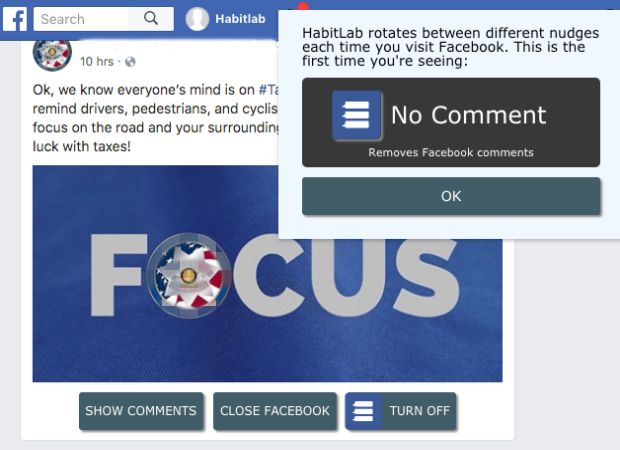
\includegraphics[width=\linewidth]{figures/info_full_facebook_new}
\caption{Mental model interface: each time the user sees a new intervention, HabitLab names it and explains about rotation.}
  \label{fig:info}
\end{minipage}
\hfill
\begin{minipage}[t]{0.49\linewidth}
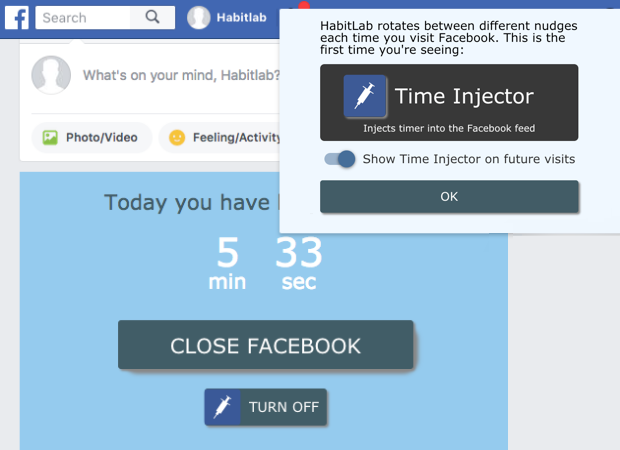
\includegraphics[width=\linewidth]{figures/power_full_facebook_new}
\caption{User control interface: in addition to the mental model information, HabitLab gives users a direct interface to disable the new intervention.}
  \label{fig:power}
\end{minipage}%
\end{figure}

%\subsection{Experimental Design}

% We ran a study comparing the ``info'' and ``power'' designs to our original system we had used in Study 1 (where the new intervention is shown without any additional messaging). An intervention was randomly selected on each visit -- the same configuration which we had found in Study 1 would increase attrition rates relative to always showing the same intervention.

\subsection{Experiment Design}

We ran a between-subjects design where we randomized the design shown to new users of HabitLab and tested whether it impacted attrition over a period of one week, similar to Study 1.

\subsection{Participants}

Our participants were HabitLab users who installed over a 10 day period in April 2018. There were a total of 282 users who installed and agreed to participate. We removed users who were not new users (e.g. an existing user installing on a new device, or a former user reinstalling the system), and users who left before they saw their first intervention. This leaves us with data from 93 participants. Demographics, estimated by Google Analytics, were similar to Study 1.

\subsection{Method}
Participants installed HabitLab and set it up as described in the Study 1 and Study 2. They used HabitLab in the course of their normal web browsing activity. HabitLab rotated between randomly chosen interventions on each visit to the chosen web page for all users, equivalent to the rotation condition in Study 1. Each time the user experienced a new intervention that they had not seen before, however, HabitLab might show an explanation design in the corner of the browser.

\subsection{Conditions}

There were three conditions for this study. %, one with no change from the last study and the other two with the new design interventions. 
%were interested in whether user retention rates would be influenced by whether or not users saw one of our two designs the first time they saw a new intervention.
%There were 3 conditions, which differ only in the design users see the first time they see a new intervention they have not previously seen. 
In the no design condition, users saw no message, equivalent to the rotation condition from Study 1. In the mental model condition, users were shown the informational intervention (Figure~\ref{fig:info}) to remind them that the system rotates interventions. In the user control condition, users were additionally given control over whether to turn off each new intervention without needing to visit the settings screen (Figure~\ref{fig:power}).

\subsection{Measures}

Our main dependent variable was attrition---how many days users kept the system installed by the end of the study, seven days after installation. The measure of attrition was the same as in Study 1 and Study 2. We also measured effectiveness, using the same method as Study 1.

\subsection{Method of Analysis}

To analyze attrition, we again used a Cox proportional hazards regression model, similar to Study 1, using interaction design as the predictor variable. To analyze effectiveness, we used a LMM predicting log time on site per day, with a fixed effect for condition, and random effects for participant and domain. Data cleaning followed the same procedures as Study 1.


%\section{Study 2 Methodology}

%Having observed in study 1 that there is an increase in attrition when alternating interventions, we sought to uncover the underlying causes. We hypothesized the following possible causes:

%\begin{enumerate}
%\item Violation of user expectations: Users may have an incorrect mental model expecting that interventions they see do not change. Even though we told them during onboarding that HabitLab will change interventions periodically, they may not have read it.
%\item Lack of control: Users may be aware that the system is choosing interventions for them, but are uncomfortable giving control to a system
%\item Seeing a new intervention reminds them that the system exists: If users grow blind to interventions over time, they may never grow sufficiently annoyed to actually bother to uninstall.
%\item Encountering bad interventions: Some users may have a particularly adverse reaction to some interventions -- simply seeing a certain intervention may lead the user to uninstall. By switching between several interventions, the user is more likely to encounter an intervention they have an intense dislike for.
%\end{enumerate}

%Reasons (3) and (4) are important -- and in fact we did observe a significant difference in attrition rates among different interventions in Study 1, confirming hypothesis (4) -- but are somewhat inevitable consequences of alternating between interventions. We also observed in informal in-person interviews that some users did not expect the system to be changing interventions. Thus, we chose to focus on addressing (1) and (2).

%We developed 2 different interfaces that aimed to address these possible violations of user expectations and provide users with a sense of control over their interventions. These interfaces were shown when users see a new intervention for the first time. The first interface, which we will call ``info'', shown in Figure \ref{fig:info}, tells the user that HabitLab rotates between different nudges. The second ``power'', shown in Figure \ref{fig:power}, shows the same message, and adds a toggle option to turn off the intervention for future visits.

%We ran a study comparing the ``info'' and ``power'' interventions to our original system we had used in Study 1 (where the new intervention is shown without any additional messaging). An intervention was randomly selected on each visit -- the same configuration which we had found in Study 1 would increase attrition rates relative to always showing the same intervention.

%\begin{figure}
%  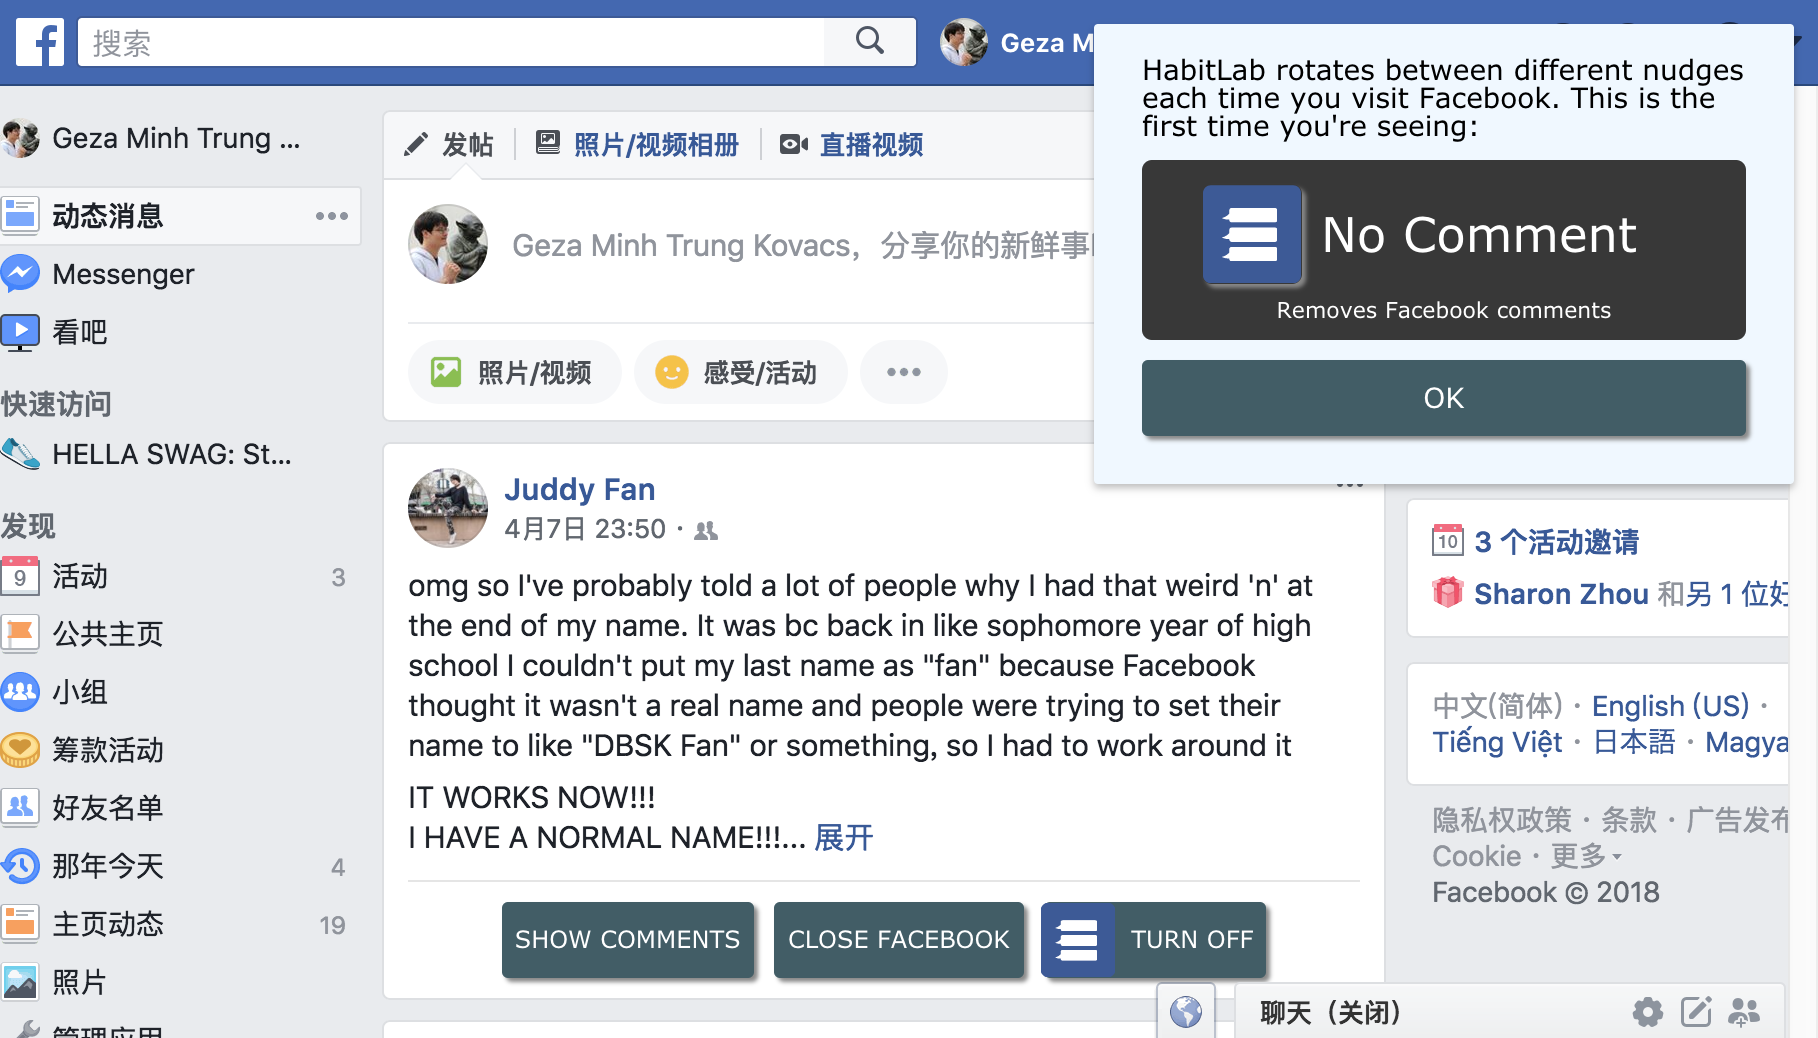
\includegraphics[width=\textwidth]{figures/info_full_facebook}
%  \caption{Interface showing info about how interventions alternate the first time a new intervention is seen.}
%  \label{fig:info}
%\end{figure}



%\begin{figure}
%  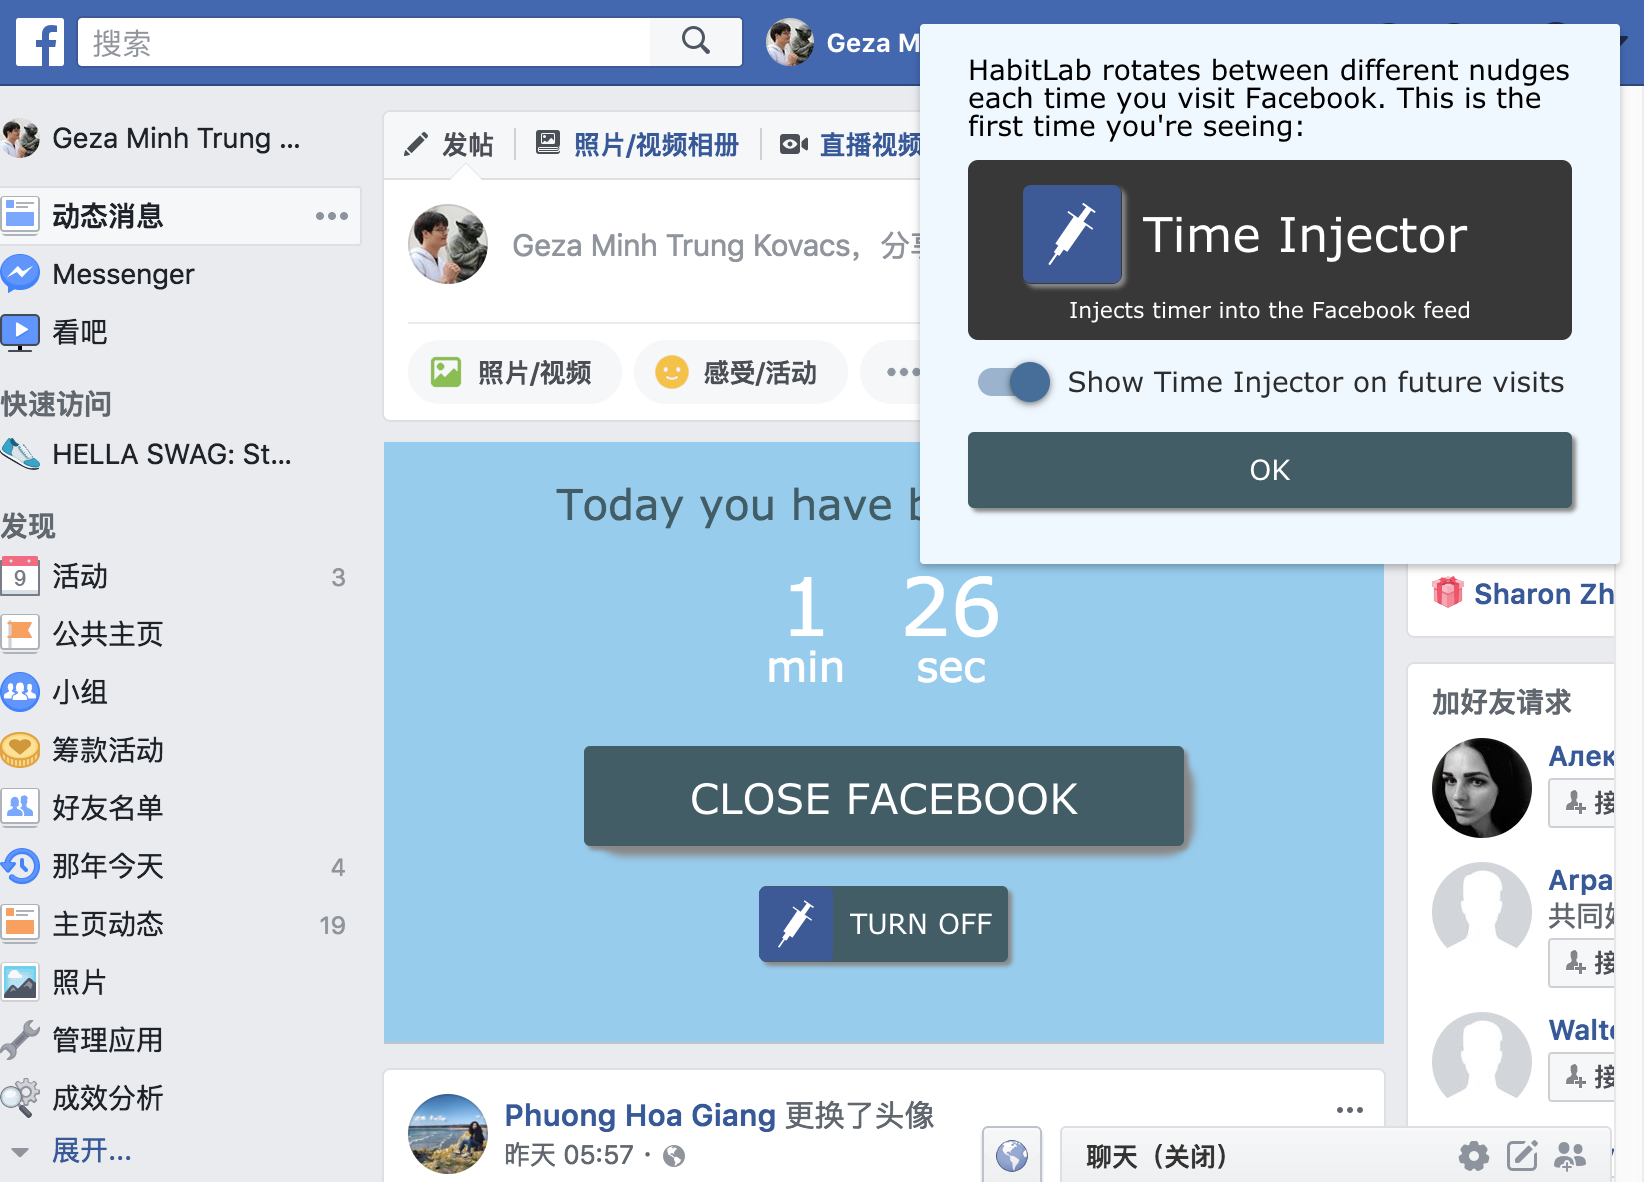
\includegraphics[width=\textwidth]{figures/power_full_facebook}
%  \caption{Interface giving users control over interventions the first time a new intervention is seen.}
%  \label{fig:power}
%\end{figure}

